% -*- coding: utf-8; -*-
% vim: set fileencoding=utf-8 :
\documentclass[english,submission]{programming}
%% First parameter: the language is 'english'.
%% Second parameter: use 'submission' for initial submission, remove it for camera-ready (see 5.1)

\usepackage[backend=biber]{biblatex}
\addbibresource{reference.bib}
\usepackage{tikz}
\usepackage{listings}
\usepackage{graphicx}
\usepackage{subcaption} % For subfigures
\usepackage{array, caption, tabularx,  ragged2e,  booktabs, xspace}



%
% Packages and Commands specific to article (see 3)
%
% These ones  are used in the guide, replace with your own.
% 
\usepackage{multicol}
\lstdefinelanguage[programming]{TeX}[AlLaTeX]{TeX}{%
  deletetexcs={title,author,bibliography},%
  deletekeywords={tabular},
  morekeywords={abstract},%
  moretexcs={chapter},%
  moretexcs=[2]{title,author,subtitle,keywords,maketitle,titlerunning,authorinfo,affiliation,authorrunning,paperdetails,acks,email},
  moretexcs=[3]{addbibresource,printbibliography,bibliography},%
}%
\lstset{%
  language={[programming]TeX},%
  keywordstyle=\firamedium,
  stringstyle=\color{RosyBrown},%
  texcsstyle=*{\color{Purple}\mdseries},%
  texcsstyle=*[2]{\color{Blue1}},%
  texcsstyle=*[3]{\color{ForestGreen}},%
  commentstyle={\color{FireBrick}},%
}

\def\iC#1{\lstinline[language=C]{#1}\xspace}

\newcommand*{\CTAN}[1]{\href{http://ctan.org/tex-archive/#1}{\nolinkurl{CTAN:#1}}}
%%

\def\coolname{\textsc{LiveRec}\xspace}

%%%%%%%%%%%%%%%%%%
%% These data MUST be filled for your submission. (see 5.3)
\paperdetails{
  %% perspective options are: art, sciencetheoretical, scienceempirical, engineering.
  %% Choose exactly the one that best describes this work. (see 2.1)
  perspective=engineering,
  %% State one or more areas, separated by a comma. (see 2.2)
  %% Please see list of areas in http://programming-journal.org/cfp/
  %% The list is open-ended, so use other areas if yours is/are not listed.
  area={Live programming, language engineering},
  %% You may choose the license for your paper (see 3.)
  %% License options include: cc-by (default), cc-by-nc
  % license=cc-by,
}
%%%%%%%%%%%%%%%%%%

%%%%%%%%%%%%%%%%%%
%% These data are provided by the editors. May be left out on submission.
%\paperdetails{
%  submitted=2016-08-10,
%  published=2016-10-11,
%  year=2016,
%  volume=1,
%  issue=1,
%  articlenumber=1,
%}
%%%%%%%%%%%%%%%%%%
\definecolor{codegray}{gray}{0.9}
\newcommand{\code}[1]{\colorbox{codegray}{\texttt{#1}}}

\definecolor{javared}{rgb}{0.6,0,0} % for strings
\definecolor{javagreen}{rgb}{0.25,0.5,0.35} % comments
\definecolor{javapurple}{rgb}{0.5,0,0.35} % keywords
\definecolor{javadocblue}{rgb}{0.25,0.35,0.75} % javadoc
 
\lstset{language=Java,
keywordstyle=\color{javapurple},
stringstyle=\color{javared},
commentstyle=\color{javagreen}}

\begin{document}

\title{\textsc{LiveRec}: Framing Debug Protocols to Hotwire Probes}
%\subtitle{Preparing Articles for Programming}% optional
%\titlerunning{Preparing Articles for Programming} %optional, in case that the title is too long; the running title should fit into the top page column

\author[a]{Jean-Baptiste Döderlein}
\affiliation[a]{ENS Rennes, Bruz, France}
\author[b]{Riemer van Rozen}
\affiliation[b]{Centrum Wiskunde \&\ Informatica (CWI), Amsterdam, The Netherlands}
\author[b,c]{Tijs van der Storm}
\affiliation[c]{University of Groningen, Groningen, The Netherlands}


\keywords{programming journal, paper formatting, submission preparation} % please provide 1--5 keywords


%%%%%%%%%%%%%%%%%%%%%%%%%%%%%
% Please go to https://dl.acm.org/ccs/ccs.cfm and generate your Classification
% System [view CCS TeX Code] stanz and copy _all of it_ to this place.
%% From HERE
\begin{CCSXML}
<ccs2012>
<concept>
<concept_id>10002944.10011122.10003459</concept_id>
<concept_desc>General and reference~Computing standards, RFCs and guidelines</concept_desc>
<concept_significance>300</concept_significance>
</concept>
<concept>
<concept_id>10010405.10010476.10010477</concept_id>
<concept_desc>Applied computing~Publishing</concept_desc>
<concept_significance>300</concept_significance>
</concept>
</ccs2012>
\end{CCSXML}

\ccsdesc[300]{General and reference~Computing standards, RFCs and guidelines}
\ccsdesc[500]{Applied computing~Publishing}

% To HERE
%%%%%%%%%%%%%%%%%%%%%%%

\maketitle

% Please always include the abstract.
% The abstract MUST be written according to the directives stated in 
% http://programming-journal.org/submission/
% Failure to adhere to the abstract directives may result in the paper
% being returned to the authors.
\begin{abstract}
  %What is the broad context of the work? What is the importance of the general research area?
  \textit{Context.}
  In the first part of his 2012 presentation ``Inventing on Principle''~\cite{InventingOnPrinciple}, Bret Victor gives a demo of live code editor for Javascript which shows the dynamic history of values of variables in real time. This form of live programming has become known as ``probes''~\cite{MakingMethodsLive,UsableLiveProgramming,ExampleBasedGraalVM}. Probes provide the programmer with permanent and continuous insight into the dynamic evolution of function or method variables, thus improving feedback and developer experience. 
  
  % What problem or question does the paper address? How has this problem or question been addressed by others (if at all)?
  \textit{Inquiry.} Although Bret Victor shows a working prototype of live probes in the context of Javascript, he does not discuss strategies for implementing them. Later work~\cite{ExampleBasedGraalVM} provides an implementation approach, but this requires a programming language to be implemented on top of the GraalVM runtime~\cite{GraalVM}. In this paper we present \coolname, a generic approach for implementing probes which can be applied in the context of many programming languages, without requiring dedicated compiler or runtime support. 
  
  % What was done that unveiled new knowledge?
  \textit{Approach.}
  \coolname is based on reusing existing debug protocols to implement probes. Methods or functions are compiled after every code change and executed inside the debugger. During execution the evolution of all local variables in the current stack frame are recorded and communicated back to the IDE for display to the user. 

  % What new facts were uncovered? If the research was not results oriented, what new capabilities are enabled by the work?
  \textit{Knowledge.}
  It turns out that debug protocols are rich enough for implementing live probes. Step-wise execution, hot code swapping, and stack frame inspection provide the right granularity and sufficient information to realize live probes, without modifying compilers or language runtimes. Furthermore, it turns out that the recently proposed Debugger Adapter Protocol (DAP)~\cite{DAP} provides an even more generic approach of implementing live probes, but, in some cases, at the cost of a significant performance penalty. 
%vRozen: "It turns out" -- heavy 'it' at start of sentence -- repetitive 2x. Suggest rephrasing: This paper establishes that ...  or simply: We show that ...

  % What argument, feasibility proof, artifacts, or results and evaluation support this work?
  \textit{Grounding.}
  We have applied \coolname to implement probes using stack recording natively for Java through the Java Debug Interface (JDI)~\cite{JDI}, and through the DAP for Java, Python, C, and Javascript, all requiring just reasonable amounts glue code. We evaluate the run-time performance of all four probes prototypes, decomposed into: compile-after-change, hotswap, single step overhead, and stack recording overhead. Our results show that live probes on top of native debug APIs are performant enough for interactive use. In the case of DAP, it depends on characteristics of the programming language.
  %vRozen: probes prototypes -- heavy alliteration -- try saying it three times fast. Suggested phrasing just 'prototypes'.
  %vRozen: 'hotswap', 'hot swap' or 'hot-swap' ?

  % Why does this work matter?
  \textit{Importance.} Live programming improves the programmer experience by providing immediate feedback about a program's execution and eliminating disruptive edit-compile-restart sequences. Probes are one way to shorten the programmer feedback loop at the level of functions and methods. Although probes are not new, and have been implemented in (prototype) systems, \coolname's approach of building live probes on top of existing and generic debug protocols opens up probes for a host of mainstream programming languages, with minimum effort.
\end{abstract}

\section{Introduction}
\label{sec:introduction}

Live programming~\cite{TanimotoLevels,UsableLiveProgramming,ExampleCentric,Hancock03} promises a better programming experience by bringing the execution of a program closer to the abstractions of the source code. By erasing the distinction between a program on the one hand, and its execution on the other, programmers may enjoy a more fluid experience, with immediate dynamic feedback after every code change.
%vRozen: 'may enjoy' ? -- Perhaps remove 'may' here.

Live programming has a rich history, both in academia and industrial research\footnote{For brief and incomplete overview of some of the history of live programming, see~\cite{LiveProgHist13}}, originating in the original Lisp systems (e.g.,~\cite{Sandewall78,Masinter81}) and Smalltalk~\cite{Goldberg80} which allowed dynamic replacement of code units (hot swapping) and inspection of program structures at run-time (sometimes referred to as ``programming in the debugger''). However, live programming became center stage after Bret Victor's influential talk ``Inventing on Principle'', which went viral in 2012. 

In that presentation Victor makes a compelling case that (paraphrasing) ``creators need to see what they are creating''. In the case of programming, this entails continuous inspection of the run-time behavior of a program, and immediate and seamless adaptation after a code change. While all the prototypes demonstrated by Victor are impressive, for the purpose of this paper we zoom in on one of them: a live editor for Javascript with a side pane showing the history of values of local function variables during an execution (see Figure~\ref{FIG:bret} below). Although not mentioned by Victor himself, this live programming features has become known as ``probes''~\cite{UsableLiveProgramming,ExampleBasedGraalVM}.
%vRozen: Singular / plural mismatch. 'these features have' or 'this feature has'. I get that 'probes' invites using the plural.
%vRozen: I'm missing a definition of probes. Probes are a specific live programming mechanism that adds immediate feedback to imperative languages, reminiscent of voltage probes, for relating the inputs of functions to their outputs.

The question left unanswered in Victor's presentation is: how to build such probes? While there has been research showcasing implementation approaches~\cite{ExampleBasedGraalVM}, they depend on a specific runtime system (e.g., GraalVM), or employ language specific ``hacks''~\cite{LiveLiterals}, and hence cannot be easily transferred to other languages. So a more specific question is: how to  engineer probes \textit{generically}, without dedicated compiler or runtime support?
%vRozen: ``hacks'' sounds a bit derogative. Let's stay friends with the reviewers :D

In this paper we present \coolname, an approach to implement probes by reusing standard debugger protocols and APIs. Most languages support an API to facilitate the implementation of debuggers and other run-time tools (e.g., profilers, tracers, etc.). It turns out that such facilities are sufficiently powerful for implementing live probes. The key to the approach of \coolname is to (re)execute a function or method inside the debugger, step by step, and at each step record a snapshot of the current stack-frame. After the method has finished executing, the resulting stack recording is communicated back to the IDE and visualized alongside the code, matching stack recording entries to the source code using source location information.
%vRozen: 'It turns out' -- heavy it.
%vRozen: 'stack-frame' or 'stack frame' ?
%vRozen: Long final sentence -- information-dense -- high mental load -- consider breaking into parts.

We first detail how to implement probes using a native debugger interface, the Java Debug Interface (JDI). Then we generalize the approach to employ the recently proposed Debugger Adapter Protocol (DAP). 
This implementation is showcased with probe implementations in Java (again), C, Python, and Javascript. 
As a result, probes can be supported in any programming language that provides an implementation of the DAP, with only a limited amount of configuration code.  

Since live programming (and hence probes) is all about immediate feedback, it is important that the performance overhead of \coolname's strategy does not impede practical use. We therefore provide a detailed analysis and measurement of the performance overhead of (re)compilation, hot-swapping, step-wise execution, and stack recording. To assess the overall usability of the approach, we furthermore decompose a full editing scenario (derived from Victor's presentation) in $19$ logical steps, replay it on every  probe implementation, and measure the performance of each edit step.
%Rozen: Repeats 'hence' -- rephrase: therefore

The contributions of this paper can be summarized as follows:
\begin{itemize}
  \item We analyze the requirements for implementing probes (Section~\ref{sec:problem-overview})
  \item We provide an overview of \coolname and introduce \textit{stack recording} as a technique to obtain the required information through standard debug protocols (Section~\ref{sec:stack-recording})
  \item We apply \coolname on top of the Java Debugger Interface (JDI) (Section~\ref{sec:live-probes-java})
  \item We then show how to generalize \coolname in the context of the Debugger Adapter Protocol (DAP) (Section~\ref{sec:generalizing-live-probes})
   \item We evaluate the feasibility of \coolname by implementing probes for Java, Python, C and Javascript on top the DAP, investigate the performance overhead of the individual steps, and reproduce an editing scenario to assess practicality (Section~\ref{sec:evaluation}).
\end{itemize}
We conclude the paper with a discussion of limitations and related work, and present concluding remarks with directions for further research. 
%vRozen: To me the paper's scientific contributions and its structure are not the same thing. The paper contributes 'stack recording', a generic approach for probes. The paper is structured as follows: ...

\section{Background and Overview}
\label{sec:problem-overview}

The basic concept of live probes is illustrated in Figure~\ref{FIG:bret}, showing two panes. 
%vRozen: 'live probes' -- \coolname?
The left pane shows an editor containing the source code of a possible implementation of binary search in Javascript. 
%vRozen: The left pane shows an editor containing JavaScript sources of an example implementation of binary search.
The right pane shows the values of variables matched up to the source line they were last updated.
%vRozen: The right pane shows the values the variables have at the source lines they were last updated.
The top two rows specify example input data that the function is executed on. 
%vRozen: Bit passive -- sentence doesn't sing -- can't put my finger on it.
The consecutive values of variables that are updated in a loop (e.g. \lstinline{low}, \lstinline{high}, \lstinline{mid} and \lstinline{value}) are displayed adjacently. 
%vRozen: Bit passive -- sentence doesn't sing -- can't put my finger on it.
So for \lstinline{low}, the history of values is 0, 3, and 5. Note that the update of \lstinline{high} in the else-if branch (apparently) never executed, so there is no (redundant) value display in the right pane. 
%vRozen: Long sentence, rephrase, remove 'so'.
Finally, the last line shows the final return value of the function: apparently the \lstinline{key} was not found in the \lstinline[language=c]{array}. 

What makes this \textit{live} is that while the programmer is editing the program on the left (or the input arguments to the function), the value display on the right continuously updates so that it is apparent what is going on at run time. 
%vRozen: Rephrase. What is 'this' ? Rephrase. This scenario exemplifies live programming. Specifically, the values displayed on the right continuously update while the programmer is editing the program on the left.

Dissecting this example leads to the following technical requirements for implementing live probes:
\begin{itemize}
  \item there should a way to specify the input arguments to a method (e.g., \lstinline{key} and \lstinline[language=c]{array});
  \item after every change to the code, it needs to be recompiled and reexecuted;
  \item during execution the values of variables needs to be recorded and linked to the source locations where they were updated.
  \item the resulting history list of values needs to be communicated to the IDE for display to the user.
\end{itemize}
%vRozen: consider starting the above sentences with a verb in simple present. Remember requirements have actors. Is that the case here? Maybe they are technical challenges.

The basic intuition of our approach to meet these requirements is as follows: the editor starts a custom debugger (implemented against some debugger API), not on the user program, but on a driver program called the Keep Alive Agent (KAA). This program consists of a while-true-loop, halted on a breakpoint, and will be the verhicle for executing methods, without having to restart the debugger upon each request. 
%vRozen: Long sentences. Consider breaking into parts. For instance: The basic intuition behind our approach is to meet these requirements as follows. Each editor starts a custom debugger, implemented against some debugger API. Instead of debugging the program directly, a this debugger runs a driver program called the Keep Alive Agent (KAA). ...

When the code changes, the editor communicates to the debugger to hotswap the code, and execute it with the input arguments extracted from the source code (based on some kind of annotation). The debugger, however, does not simply execute it, but simulates execution by issuing step-over commands until the method completes. To keep stack recording local to the current method, the debugger never steps \textit{into} a call to another method.
%vRozen: 'hotswap', 'hot swap' or 'hot-swap' ?
%vRozen: 'some kind' -- vague -- a particular ?

In between steps, the debugger takes snapshots of the current stack frame to record the values of local variables.  These snapshots are stored in a data structure, called \textit{stack recording}, which supports displaying the values in the IDE, for instance, like in Figure~\ref{FIG:bret}, inline~\cite{LiveLiterals,ExampleBasedGraalVM}, or using some dedicated UI affordance. 
%vRozen: Long sentence. Consider breaking into parts. ", which supports displaying the values in the IDE." 
%vRozen: For example, Figure ...
%vRozen 'some dedicated' -- vague -- replace 'some' by 'a'

\begin{figure}[t]
  \centering
  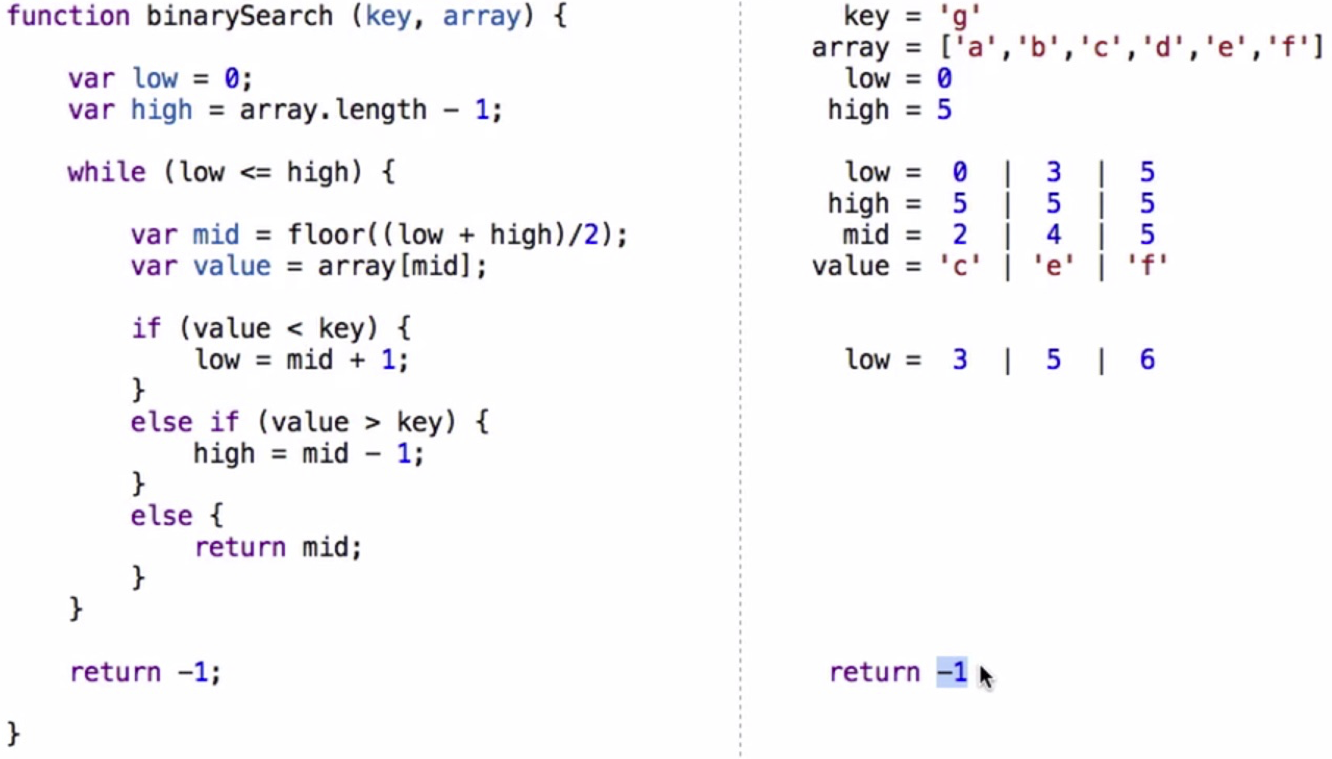
\includegraphics[width=\textwidth]{img/bret}
  \caption{Screenshot of Bret Victor's 2012 talk ``Inventing on Principle'' (23rd minute)~\cite{InventingOnPrinciple}}
  \label{FIG:bret}
\end{figure}


\section{Using the Debugger ?}
%vRozen: todo fixme heading title

\subsection{Architecture}

\begin{figure}[h]
  \centering
  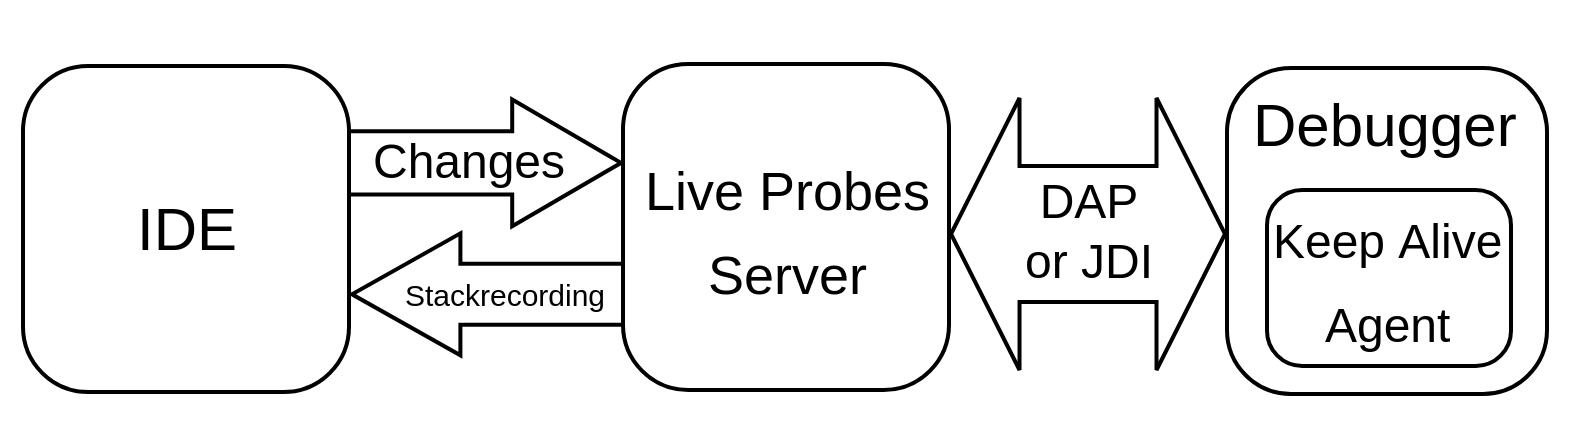
\includegraphics[width=0.8\linewidth]{img/architecture.png}
  \caption{General architecture (placeholder)}
  \label{fig:architecture}
\end{figure}
%vRozen: todo fixme remove 'placeholder'
%vRozen: perhaps a tikz image here

A live environment must be able to react to two different events: a change in the code or a change in the test/input data. 
%vRozen: 'live environment' -- 'live programming environment'
If the code changes, we need to re-execute the code, and in the case of a compiled language, we need to compile the new code first. 
%vRozen: who is 'we' ? Consider replacing 'we' by 'a programmer' Whenever a programmer changes the code, ...
If the data changes, we need to be able to re-execute the programme with the new data. 
%vRozen: Likewise, the program needs to re-execute immediately when the programmer adjusts the inputs.
In addition, it is necessary to keep compilation and execution times low enough to maintain an interactive experience with the user.
%vRozen: 'the user' -- suggest 'the programmer' or 'programmers'

To meet these constraints, we propose the architecture shown in Figure \ref{fig:architecture} :
\begin{itemize}
  \item The IDE or editor communicates with a server. The IDE sends changes to the code and function parameters, and the server sends back the stack trace of the method.
%vRozen: 'or'. The editor is part of an IDE that ...
  \item The server initialises and communicates with the debugger to apply the changes received from the IDE, and generates a stack recording when the method is executed.
%vRozen: US English: Initializes
%vRozen: The server initializes the debugger, and continually applies the changes it receives from the IDE, generating a stack recording when a method is executed.
  \item The debugger runs an intermediate program, a keep alive agent. This keeps the debugger alive to reduce initialisation times.
%vRozen: Note -- The acronym Keep Alive Agent (KAA) has been introduced already.
%vRozen: The debugger runs the Keep Alive Agent, an intermediate program for reducing initialization times, which keeps the debugger alive between executions.
\end{itemize}

\label{sec:stack-recording}
%vRozen: fixme dangling label

\subsection{Stack Recording}

\begin{figure}[h]
  \centering
  \begin{minipage}{0.25\textwidth}
    \centering
    \begin{lstlisting}[language=C]
//foo(3)
int foo(int n) {
  int i = 0;
  while (i < n) {
    i++;
  }
  return i;
}
    \end{lstlisting}
  \end{minipage}
  \hfill
  \begin{minipage}{0.7\textwidth}
    \centering
    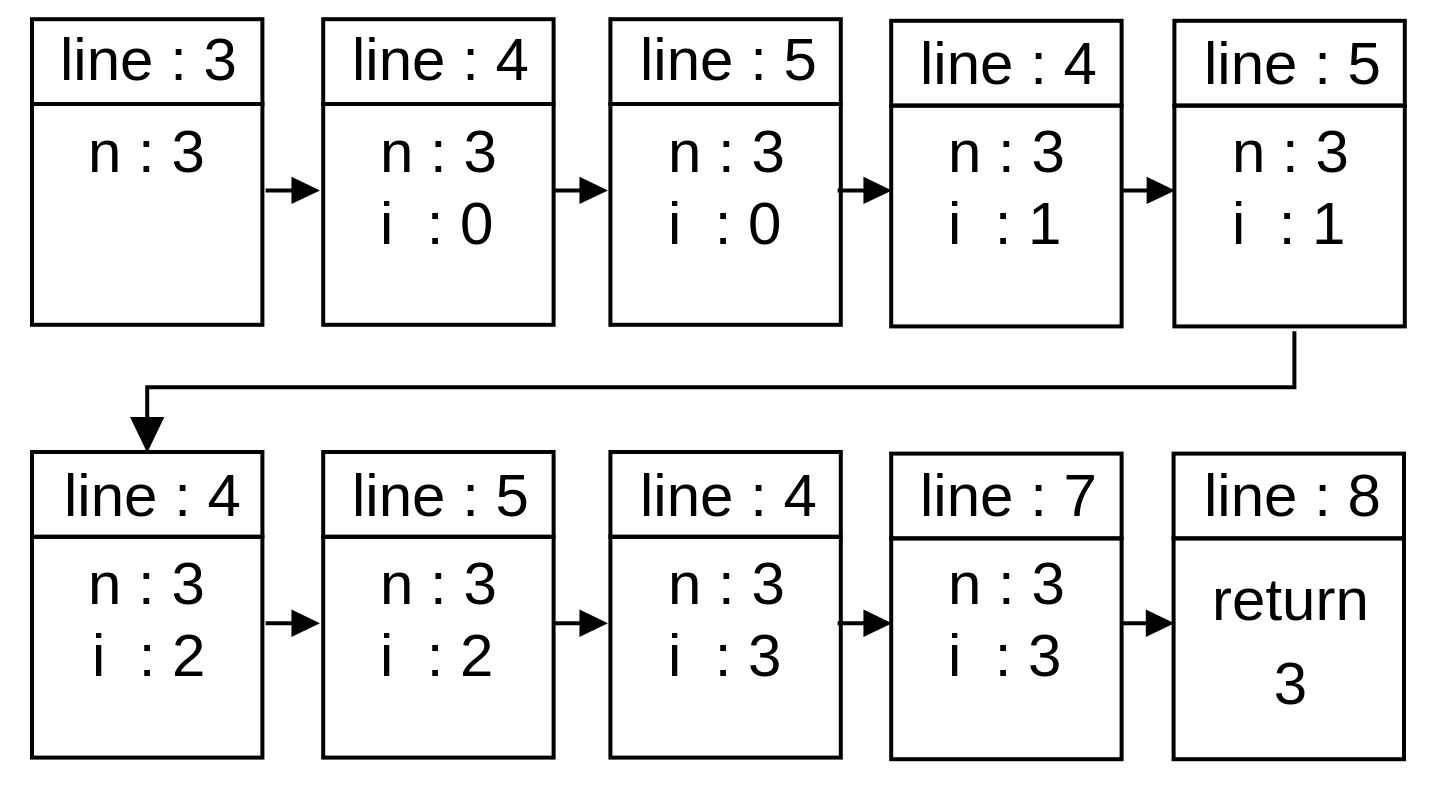
\includegraphics[width=0.8\linewidth]{img/stackrecording_chain.png}
  \end{minipage}
  \caption{Stack Recording Example}
  \label{fig:stack-recording}
\end{figure}
%vRozen. The layout seems a bit off.

\begin{table}[t]
  \centering
  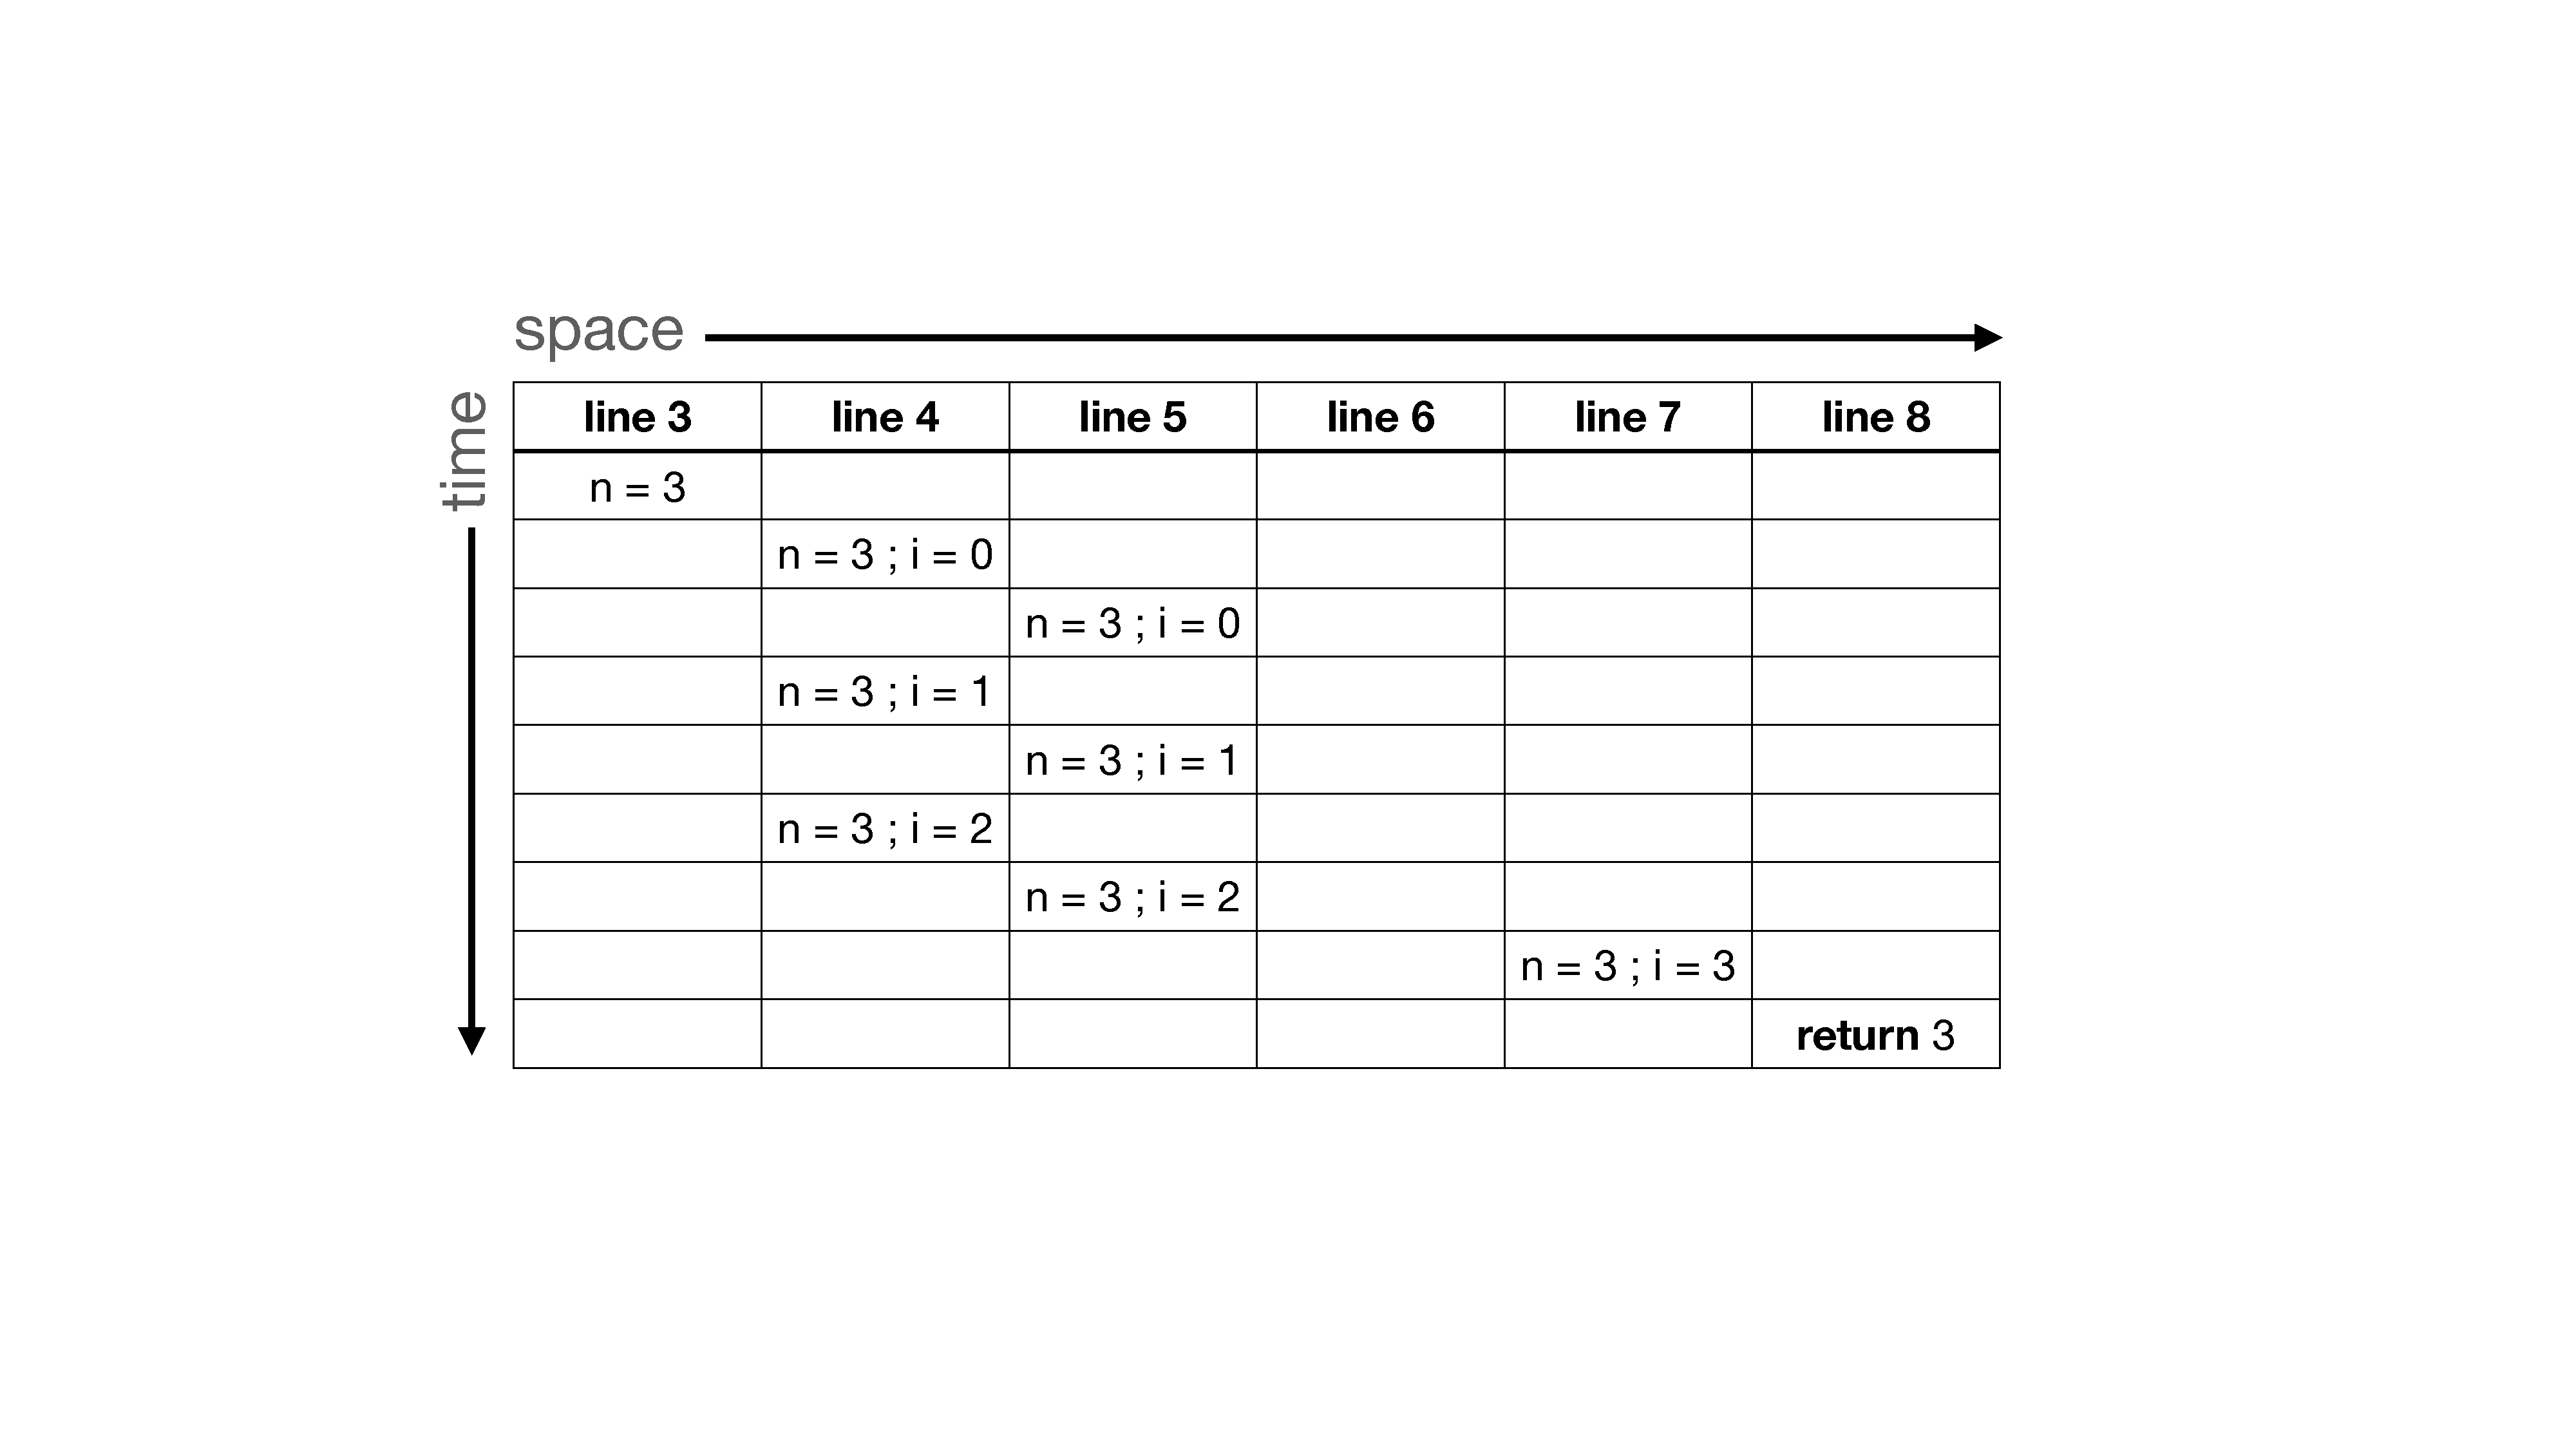
\includegraphics[width=\textwidth]{img/matrix.pdf}
  \caption{Tracking variable values across time and space}
\end{table}


\begin{figure}
  \centering
  \large  
  \hspace{8pt} \color{darkgray} \textsf{\textbf{time}}  \color{black} $\rightarrow$ \raggedright
  \vspace{2pt}
   
  \rotatebox{90}{$\leftarrow$ \color{darkgray} \textsf{\textbf{space} \color{black}}}
  \small
  \begin{tabularx}{0.94\textwidth}{ l @{\hspace{4pt}} l @{\hspace{4pt}} X @{\hspace{4pt}} X @{\hspace{4pt}} X @{\hspace{4pt}} X @{\hspace{4pt}} X @{\hspace{4pt}} X @{\hspace{4pt}} X @{\hspace{4pt}} X @{\hspace{4pt}} X @{\hspace{4pt}} X @{\hspace{4pt}} l}  
  \toprule  
  &
  &
  \textbf{$t_1$}&
  \textbf{$t_2$}&
  \textbf{$t_3$}&
  \textbf{$t_4$}&
  \textbf{$t_5$}&
  \textbf{$t_6$}&
  \textbf{$t_7$}&
  \textbf{$t_8$}&
  \textbf{$t_9$}\\
  \midrule
  &
  &
  \iC{n; i} &
  \iC{n; i} &
  \iC{n; i} &
  \iC{n; i} &
  \iC{n; i} &
  \iC{n; i} &
  \iC{n; i} &
  \iC{n; i} &
  \iC{n; i} \\
  \midrule
  1 & \iC{//foo(3)}\\
  2 & \iC{int foo(int n)\{} \\
  3 & \hspace{8pt}~\iC{int i = 0;}
  & \iC{3; _} \\  
  4 & \hspace{8pt}~\iC{while(i < n)\{} 
  &
  & \iC{3; 0}
  &
  & \iC{3; 1}
  & 
  & \iC{3; 2}\\
  5 & \hspace{16pt}~\iC{i++;}
  &
  &
  & \iC{3; 0}; 
  &
  & \iC{3; 1}\\
  6 & \hspace{8pt}~\iC{\}}\\
  7 & \hspace{8pt}~\iC{return i;}
  &
  &
  &
  &
  &
  &
  &
  &
  \iC{3; 3}\\
  8 & \iC{\}}
    &
  &
  &
  &
  &
  &
  &
  &
  &
  \iC{return 3}\\
  \bottomrule
  \end{tabularx}
  \caption{Tracking variable values across time and space}
\end{figure}



% \begin{table}[ht]
%   \centering
%   \begin{tabular}{|c|c|c|c|c|}
%   \hline
%       \textbf{Line 3} & \textbf{Line 4} & \textbf{Line 5} & \textbf{Line 7} & \textbf{Line 8} \\ \hline
%       n=3 & n=3;i=0 & n=3;i=0 & ~ & ~ \\ \hline
%       ~ & n=3;i=1 & n=3;i=1 & ~ & ~ \\ \hline
%       ~ & n=3;i=2 & n=3;i=2 & ~ & ~ \\ \hline
%       ~ & n=3;i=3 & ~ & n=3;i=3 & return 3 \\ \hline
%   \end{tabular}
%   \label{tab:stack-recording}
%   \caption{Stack Recording Example 2}
% \end{table}

In order to generate the data needed to probe a variable, we need to be able to retrieve the state of the variable during execution. 
This information is contained in the stackframe at the time of execution. 
However, we need to add spatial and temporal information to this: we need to associate each stackframe state with the location in the code at which it was retrieved, and we also need to know the order in which these stackframes were retrieved.

In this paper, we introduce a structure for representing this data: a \textit{stack recording}. 
A stack record represents the different states of the stack frame during the execution of a method. The stack record is presented as a chain of recorded stack frames, to which information has been added about the source code's location and height in the stack.
This representation allows us to maintain a link between the spatial location (the reference to the source code) and the temporal location (the order of these stackframes) of the execution.
This representation has several advantages: it is easy to construct from debugger information, and it applies to most programming languages.
Figure \ref{fig:stack-recording} shows an example of a stack recording. On the left is a C function and on the right is the stack recording of the execution of \code{foo(3)}. Each rectangle represents the state of the stackframe during execution, with the source code location (here simplified to the line number).

\begin{figure}[h]
  \centering
  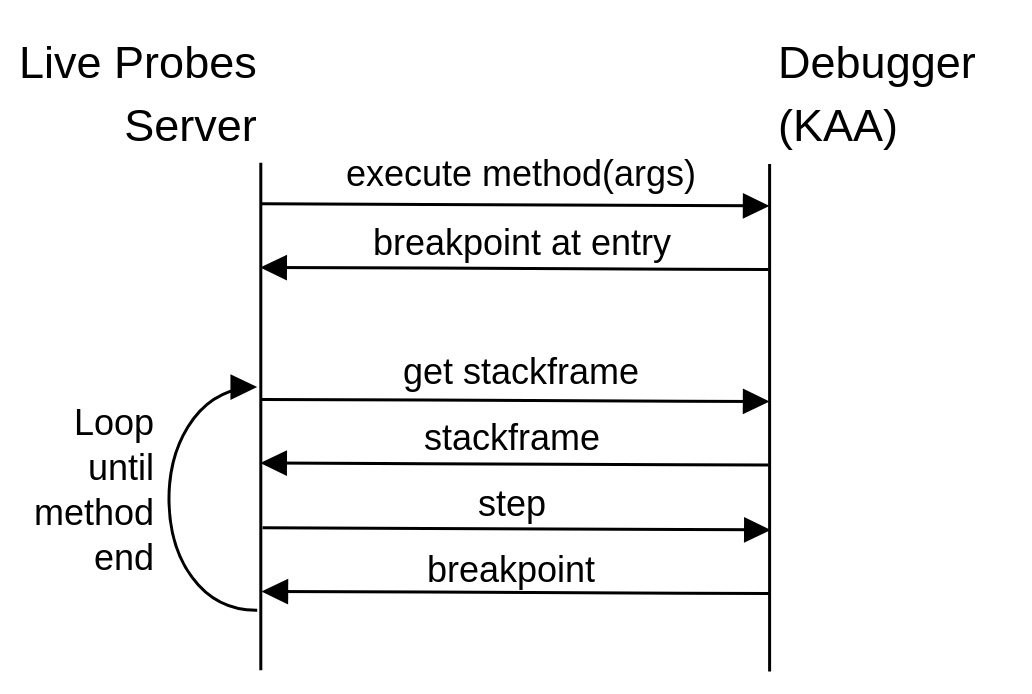
\includegraphics[width=0.6\linewidth]{img/stackrecording_impl.png}
  \caption{Record Stackrecording (placeholder)}
  \label{fig:stack-recording-impl}
\end{figure}

Figure \ref{fig:stack-recording-impl} shows how a stack recording is recorded.
To obtain the different states of the stackframe during the execution of a method, we place a breakpoint at the start of the function. 
Once this has been reached, the method is executed step by step, using the debugger's step instruction. 
Between each step, the state of the stackframe is recorded along with the source code's location information.


\section{Live Probes in Java with JDI}
\label{sec:live-probes-java}
% listing of a java class
\begin{figure}[htbp]
  \centering
  \begin{lstlisting}[language=Java]
public class LiveProbesServer{
  LiveProbesServer()
    this.kaa = new KeepAliveAgent();
  }

  public void run(){
    setBreakpointOnWhileTrue();
    launchVM(kaa);
  }
  public void loadClass(className){
    kaa.loadClass(className);
  }

  public StackRecording execute(method, arguments){
    createMirrorArguments(arguments);
    setBreakpointAtMethod(method);
    invokeMethod(method, arguments);
    stackRecording = new StackRecording();
    while(!isMethodFinished()){
      stackRecording.add(getStackFrame());
      stepDebuggee();
    }
    return stackRecording;
  }
}
  \end{lstlisting}
  \caption{Live Probes Server ?}
  \label{fig:debugger-class}
\end{figure}

\begin{figure}[htbp]
  \centering
  \begin{lstlisting}[language=Java]
public class KeepAliveAgent {
  DynamicClassLoader dynamicClassLoader;

  public void loadClass(String className){
    dynamicClassLoader.loadClass(className);
  }

  public static void main(String[] args){
    while (true) {}
  }
}
  \end{lstlisting}
  \caption{JDI Keep Alive Agent}
  \label{fig:java-keep-alive-agent}
\end{figure}

To enable stack recording, we developed a debugger leveraging the Java Debug Interface (JDI) library. 
A simplified pseudo-code representation of this debugger is displayed in Figure \ref{fig:debugger-class}. 
The class contains a method for starting the JVM (at line 2), a process to load or reload a class within the VM (at line 5), and a procedure for generating a method stack record (at line 10). Although in practice, the implementation involves multiple interacting threads, these details have been omitted from this overview in favor of clarity and simplicity.

Initialization involves the launch of a JVM that features JDI instrumentation, utilizing the KeepAliveAgent class (in Figure \ref{fig:java-keep-alive-agent}). 
Concurrently, a breakpoint is established at the infinite loop within the \code{main} function, visible at line 9. 
This breakpoint's function is to maintain the debugger in a state of suspension. This waiting state is requisite for the use of JDI primitives such as \code{mirrorOf}, \code{newInstance}, and \code{invokeMethod}.

Class loading is achieved using a dynamic ClassLoader, which gives us the ability to append class paths and load a class during execution. 
Modifications to the code cause the class to be reloaded into the KeepAliveAgent. 
However, there is a caveat to this procedure - it only works if the class signature remains consistent and only the method content is changed. 
Any changes to the structure will require a restart of the KeepAliveAgent. 
It is to be noted that specific JVM implementations can bypass this limitation \cite{}.

To execute a function (line 10 in Debugger class, Figure \ref{fig:debugger-class}), the debugger creates the values associated with the arguments locally. 
It then transmits these values to the JVM containing the KAA using the \code{mirrorOf} and \code{newInstance} methods of JDI's Reflection API (line 11). 
The debugger then sets a breakpoint at the target method's input (line 12) and launches the target method using \code{invokeMethod}. 
The debugger then registers the stack using the algorithm described in the previous paragraph.
Until the method is completed, the debugger registers the stack frame and takes a step forward in debugging.

\section{Generalizing Live Probes with Debugger Adapter Protocol}
\label{sec:generalizing-live-probes}
The Debug Adapter Protocol (DAP), developed by Microsoft, is a standard method of communicating with a programming language debugger. It is compatible with various editors, including VS Code, and provides a unified interface for all programming languages. 

By exploiting this protocol, we have created a new language parametric backend, which we have implemented for the C, Python, Java and Javascript programming languages. These languages are chosen to cover both compiled and interpreted languages. 
This backend offers an interface common to all three languages, which includes methods for starting and initialising the debugging server, loading and reloading code in the debugger, and executing a method while performing stack recording. 
Table \ref{tab:dap-req} contains a list of the requests from the DAP that we have used to implement the interface.

\begin{table}[h]
  \centering
  \noindent\setlength\tabcolsep{4pt}%
  \begin{tabularx}{\linewidth}{ll*{2}{>{\RaggedRight\arraybackslash}X}}
    \toprule
    Request & Usage \\ [0.5ex]
    \midrule
    Initialize and Launch & Initialize the DAP server and launch the debuggee \\ 
    \addlinespace
    SetBreakpoints & Set breakpoints at location in source code \\ 
    \addlinespace
    StackTrace & Get the state of the current stacktrace \\ 
    \addlinespace
    Scops and Variables & Get the current scopes and variables in it \\ 
    \addlinespace
    Evaluate & Evaluate expression in the debugee \\ 
    \addlinespace
    Next and Continue & Request to step or continue in the debuggee \\ 
    \addlinespace
    \bottomrule
  \end{tabularx}
  \caption{DAP Requests}
  \label{tab:dap-req}
\end{table}

These methods allow us to carry out stack recording independently of the chosen language and facilitate the future implementation of live programming interfaces. 

The implementation for each language includes a keep-alive agent and code to communicate with the debugger and keep-alive agent to provide the interface functionality.
These methods depend on both the implementation of the debugging server and the keep-alive agent. The differences between the implementations are shown in the Table \ref{tab:implementation-differences}.


\begin{table}[h]
    \centering
    \noindent\setlength\tabcolsep{4pt}%
    \begin{tabularx}{\linewidth}{lc*{4}{>{\RaggedRight\arraybackslash}X}}
      \toprule
      Implementation & Compile & Load Code & Execution Caller \\ [0.5ex]
      \midrule
      JDI Java & Java Compiler API & Dynamic ClassLoader & Debugger \\ 
      \addlinespace
      DAP Java & \code{javac} from command line & Dynamic ClassLoader & Debuggee \\ 
      \addlinespace
      DAP Python & ~ & Interpreted in debug console & Debuggee \\ 
      \addlinespace
      DAP C & \code{gcc} from command line & Loaded as shared library & Debugger \\
      \addlinespace
      DAP Javascript & ~ & Imported as module & Debuggee \\ 
      \bottomrule
    \end{tabularx}
    \caption{Implementation differences between languages}
    \label{tab:implementation-differences}
\end{table}

With DAP, the compilation step is performed by calling a command line compilation tool (javac and gcc). For the JDI version, developed in Java, the Java compilation API has been used for better performance.

The way the code is loaded also depends on the programming language. For Python, the code is loaded by being interpreted by the debug console during execution.
For Javascript, a line is added at the end of the imported file to export all the functions in the file as a module, which is then loaded into the KeepAliveAgent with \code{require}.
For Java, as with the JDI version, a Dynamic ClassLoader is used. For C, the code is loaded into shared libraries that can be added and reloaded at runtime.

Method execution can be divided into two categories.
For Java with DAP, Python and Javascript, calling methods directly from the debugger does not trigger breakpoints. To remedy this, execution must be initiated by the KeepAliveAgent rather than by a debugger command. 
To do this, the KeepAliveAgent code in these languages has fields for referencing a method and its arguments; when this information is entered, the agent starts execution.
In C, as in Java with JDI, the method is called from the debugger console.

\subsection{Implementation specifications}

\begin{table}[!ht]
  %\centering
  \noindent\setlength\tabcolsep{4pt}%
  \begin{tabular}{lrlrl}
      \toprule
      Implementation & \multicolumn{2}{l}{\#SLOC Probe Server} & \multicolumn{2}{l}{\#SLOC Keep-Alive Agent} \\
      \midrule
      Java JDI & 521 & Java & 75 & Java \\ 
      DAP Base & 270  & Python & --- & \\ 
      DAP Python & 142 & Python & 26 & Python \\ 
      DAP Java & 360 & Python & 114 & Java \\ 
      DAP Javascript & 256 & Python & 24 & Javascript \\ 
      DAP C & 181 & Python & 14 & C \\
      \bottomrule
  \end{tabular}
  \caption{Size of the language specific components in SLOC and their implementation languages.}
  \label{tab:sloc}
\end{table}

The table \ref{tab:sloc} shows the number of lines of code for the server part and the KAA for each implementation, with the language in brackets. The DAP Base line corresponds to the common code used by the other DAP-based implementations.
The tests were carried out with OpenJDK 20.0.2 for Java, Python 3.11.2 for Python and Node 18.16.1 for Javascript. The C code was compiled using GCC 13.1.1 and GDB 13.2 was used for stack recording. The machine used to carry out the evaluations has an AMD Ryzen 5 2500U CPU and 8Gb of RAM.

\section{Evaluation}
\label{sec:evaluation}
\subsection{Demo : A Minimal Live Programming Environment}
\label{sec:demo-small-c}


We have developed a dynamic programming environment that integrates live probes via Java, C, Python and Javascript debugging servers. 

Each time changes are made in the code editor, the code is sent to the server, which then checks for parseability and syntax errors. 
In addition, if the code contains a comment beginning with "@", followed by a function call, the server attempts to create a stack recording of that function, with the parameters provided. 

The user interface consists of a web page that interacts with a local server. The demo features two display methods. 

\subsubsection{Bret Victor's style}
\label{sec:bret-victor-style}
\begin{figure}[htbp]
  \centering
  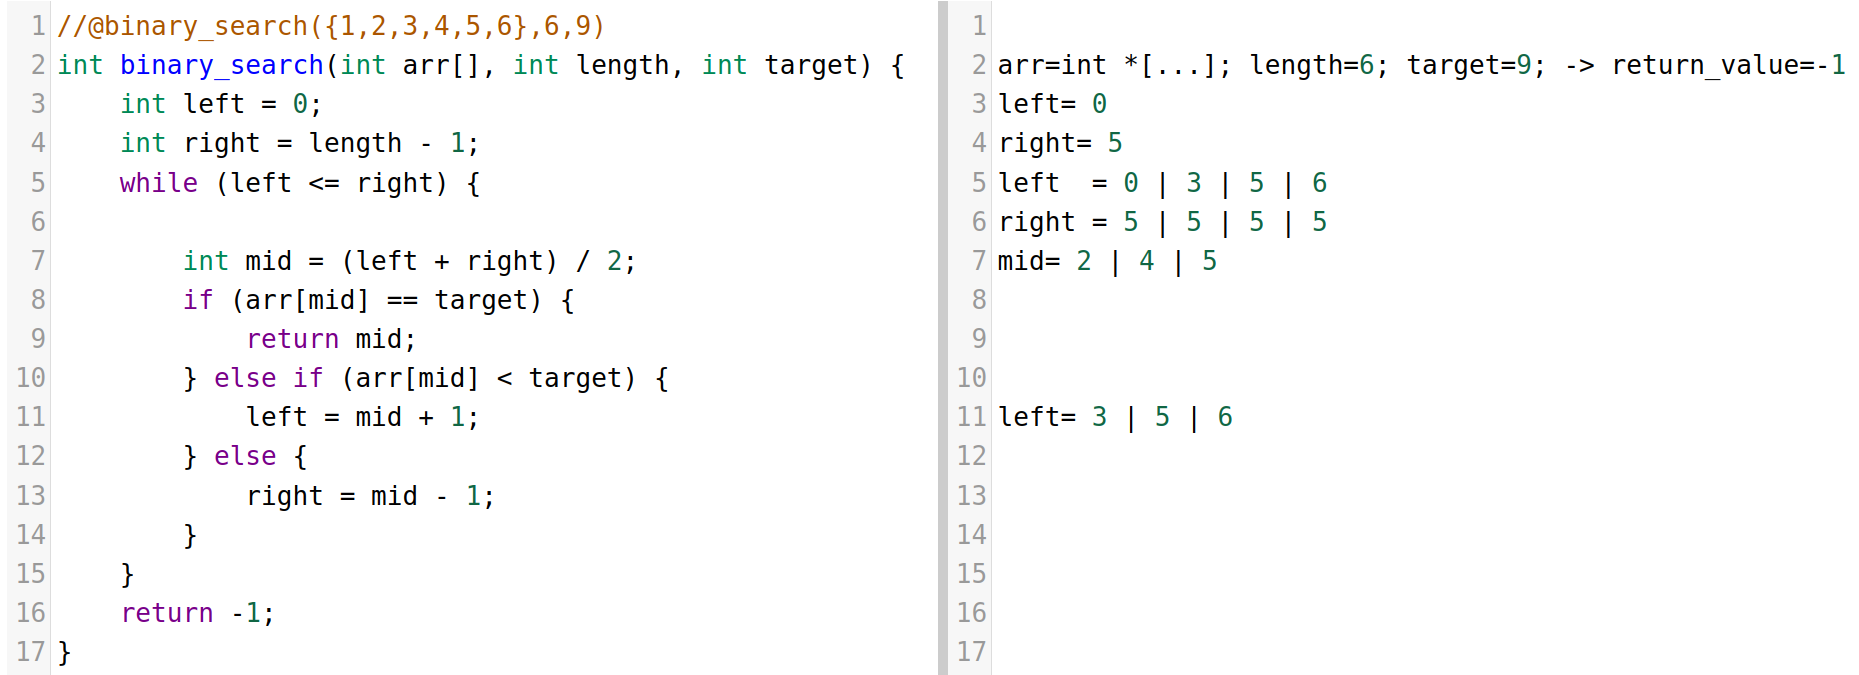
\includegraphics[width=\linewidth]{img/demo/c.png}
  \caption{Demo of the live programming environment for C.}
  \label{fig:demo}
\end{figure}

The first mode is inspired by Bret Victor's presentation. The screenshot in Figure \ref{fig:demo} shows a session with a C binary search function. 
On the left side there is a code editor (based on CodeMirror 5), while on the right a panel displays live probes. The display on the right is generated from source code and stackrecording with a tree sitter to display probes in different locations: 

\begin{itemize}
  \item Display of input arguments and return values for each function call.
  \item Displays the value of each variable definition or assignment. In cases where the assignment is in a loop or is called several times, all the different values are displayed.
  \item Display comparison values for each loop (for and while).
\end{itemize}

The use of the tree-sitter is not required to display probes. In fact, it could simply display the variables when they are modified. However, using the tree sitter also allows us to be able to display the state of variables where they are used, such as in comparisons in loops.

\subsubsection{Stack explorer}

\begin{figure}[htbp]
  \centering
  \begin{subfigure}[b]{0.45\textwidth}
      \centering
      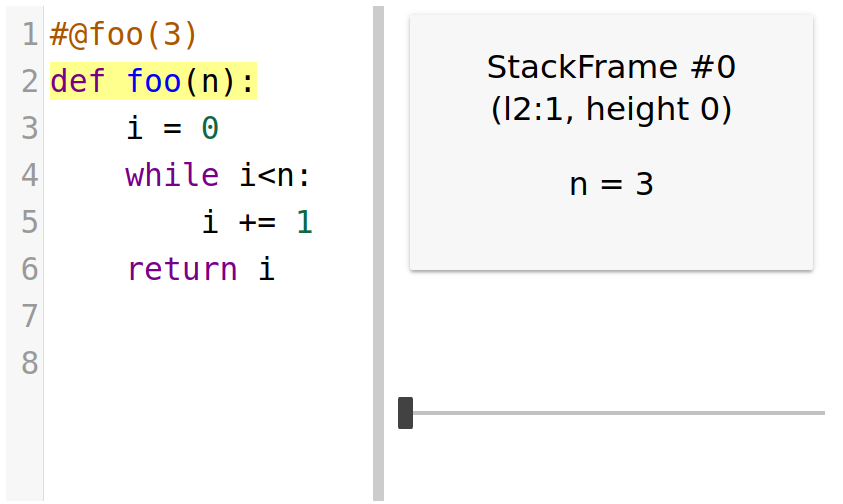
\includegraphics[width=\textwidth]{img/demo/stack/0.png}
  \end{subfigure}
  \hfill
  \begin{subfigure}[b]{0.45\textwidth}
    \centering
    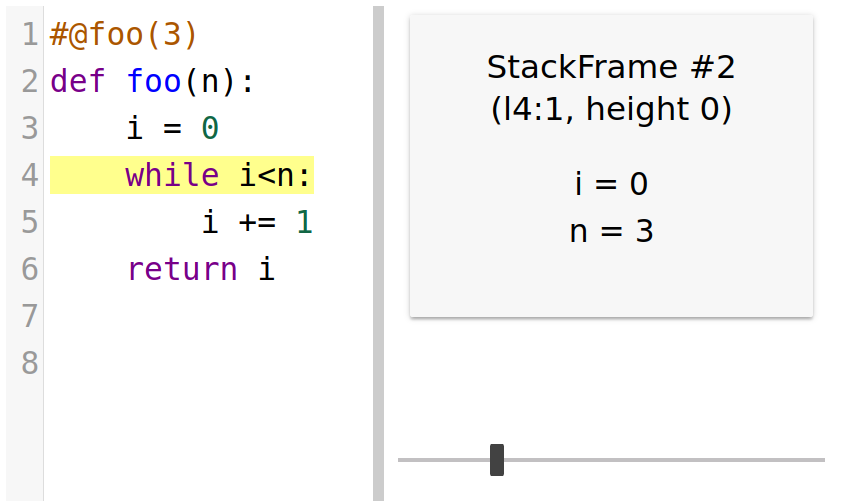
\includegraphics[width=\textwidth]{img/demo/stack/1.png}
  \end{subfigure}
  \vfill
  \par\bigskip
  \begin{subfigure}[b]{0.45\textwidth}
    \centering
    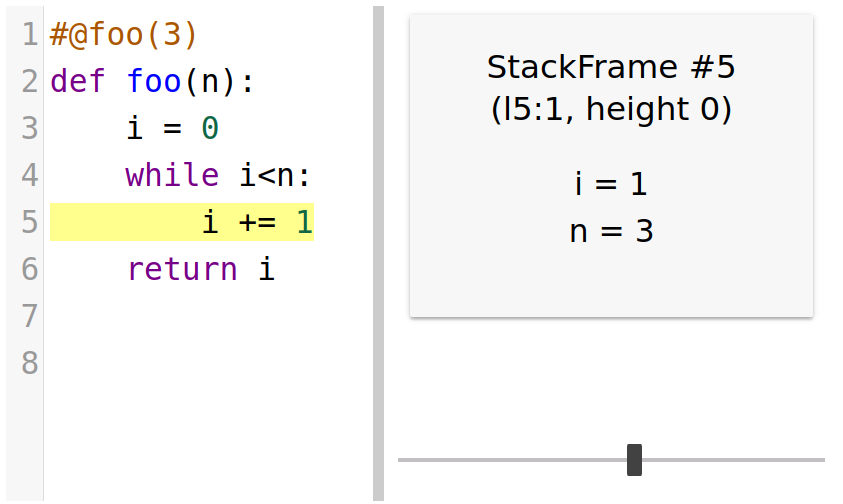
\includegraphics[width=\textwidth]{img/demo/stack/2.png}
  \end{subfigure}
  \hfill
  \begin{subfigure}[b]{0.45\textwidth}
    \centering
    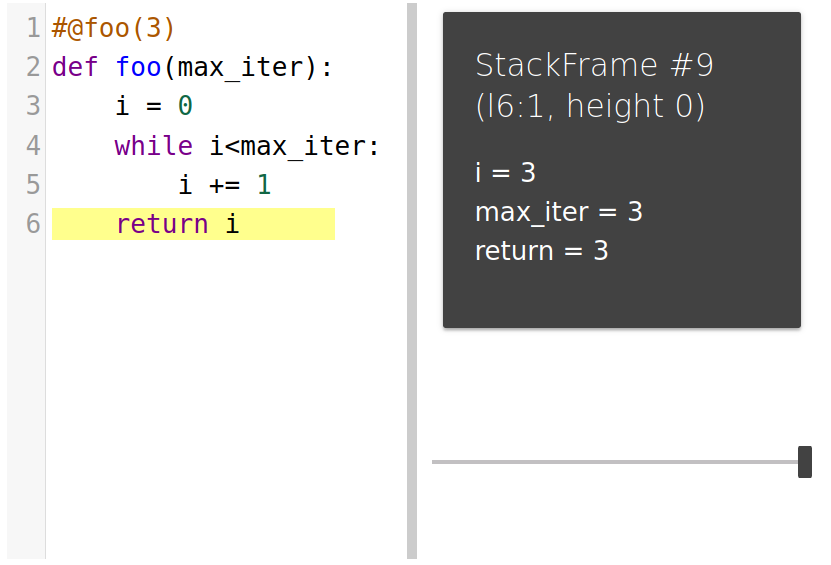
\includegraphics[width=\textwidth]{img/demo/stack/3.png}
  \end{subfigure}
  \caption{Demo of stack explorer}
  \label{fig:demo-stack}
\end{figure}

The second mode, featured in Figure \ref{fig:demo-stack}, displays the stack recording in the form of a history. The screenshots show the different stack states recorded. The right-hand panel shows the stackframe state and a slider for exploring the different states. The location in the source code corresponding to the state where the stackframe has been registered is highlighted in yellow in the Codemirror editor on the left.

\subsection{Performance}
\label{sec:performance}

In the context of a live programming environment, it is essential to have short response times after user interactions. 
We therefore measured the performance of our approach in response to various questions:

\begin{itemize}
  \item How long does it take to compile and to load the code into the debugger, depending on the size of the programme?
  \item How long does it take to run the program, depending on the number of stack frames needed to make the stack recording?
  \item What is the average performance during a live programming session?
\end{itemize}

\subsubsection{How long does it take to compile and to load the code into the debugger, depending on the size of the programme?}

\begin{figure}[htbp]
  \centering
  \begin{subfigure}[b]{0.48\textwidth}
      \centering
      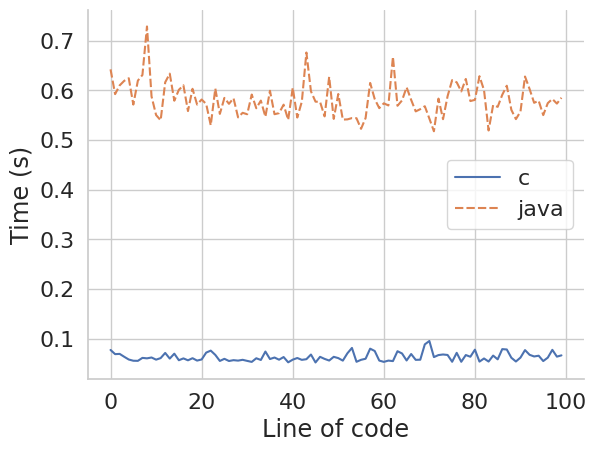
\includegraphics[width=\textwidth]{img/compile_code.png}
      \caption{\centering Compile code time}
      \label{subfig:compile}
  \end{subfigure}
  \hfill
  \begin{subfigure}[b]{0.48\textwidth}
      \centering
      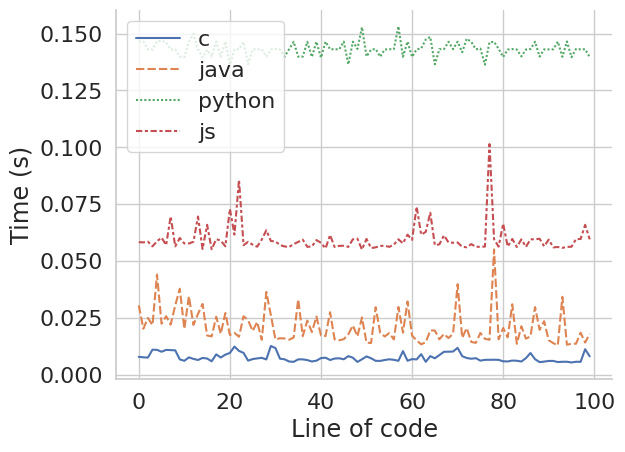
\includegraphics[width=\textwidth]{img/load_code.png}
      \caption{\centering Load code time}
      \label{subfig:load}
  \end{subfigure}
  \caption{Compile and load code time depending on the number of lines of code.}
  \label{fig:compileload}
\end{figure}

In our evaluation, we assessed the time required to compile and load code into the debugger memory for Python, C, Java and Javascript. 
To accomplish this, we compiled and loaded programs ranging from 5 to 100 lines of code. 
The summarized results can be found in Figure \ref{fig:compileload}.

In Sub-figure \ref{subfig:compile}, we present the compilation time for C and Java based on the number of lines of code. 
The compilation process was executed from the command line using javac and gcc. 
The compilation times remain nearly constant, regardless of the number of lines of code, with an average of 34.6 ms for Java and 8.5 ms for C.

Moving to Sub-figure \ref{subfig:load}, we depict the loading time in the debugger for C, Java, Python and Javascript as a function of the number of lines of code. 
The data shows that the loading time remains constant concerning the number of lines of code. 
%On average, Python takes 3 ms, Java takes 2.8 ms, and C takes 1 ms for loading.

\subsubsection{How long does it need to run the program, depending on the number of steps to make the stack recording ?}

\begin{figure}[htbp]
  \centering
  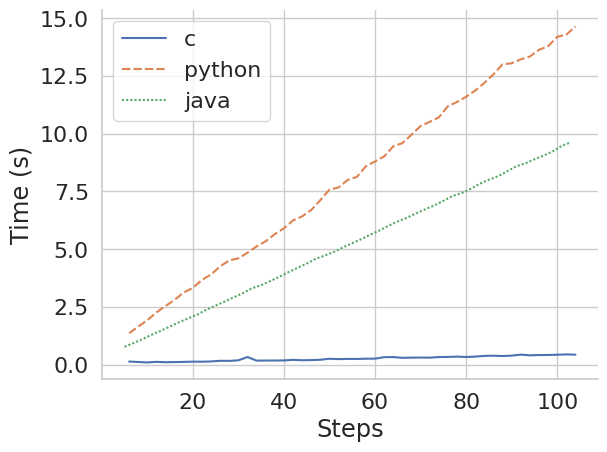
\includegraphics[width=0.5\textwidth]{img/execute.png}
  \caption{Execution time with DAP in seconds depending on the number of steps.}
  \label{fig:execute-time}
\end{figure}

\begin{figure}[htbp]
  \centering
  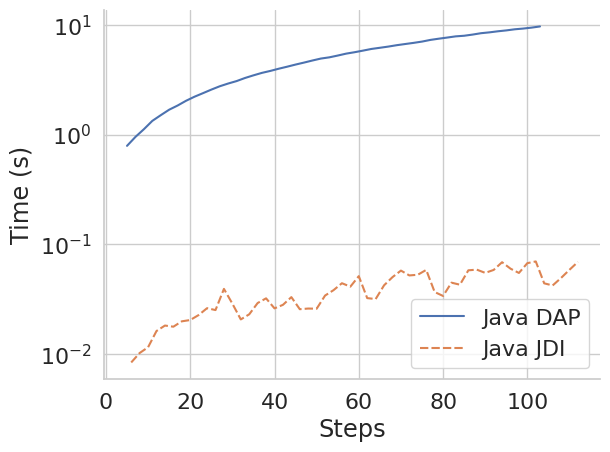
\includegraphics[width=0.5\textwidth]{img/execute_java_jdi.png}
  \caption{Comparison of execution time with DAP and JDI in seconds depending on the number of steps.}
  \label{fig:execute-java-jdi}
\end{figure}

Next, we evaluated the execution time as a function of the number of steps in the debugger. 
Figure \ref{fig:execute-time} shows the total time taken as a function of the number of steps during stack registration.
Note that the execution time shows a linear relationship with the number of steps in the method. 
In fact, for each implementation we obtain a constant time for each stack frame recorded, corresponding to the time taken to obtain the state of the stack frame and the time taken for the debugger to perform a step. 
The difference in time between the different DAP languages is explained by the implementation of the debug server. 
With C, the debug server is a simple wrapper around gdb, which has very good performance.
Figure \ref{fig:execute-java-jdi} shows Java execution times with DAP and JDI. 
The y-axis is in logarithmic scale. 
There is a significant difference in performance between the two implementations, despite the fact that the DAP server implementation in Java also uses JDWP.
By profiling the execution of the java debug server, we found two causes for this performance gap:
\begin{itemize}
  \item The first is due to the "evaluate" request in the DAP protocol. To run the function and define the arguments in the DAP implementation, we use "evaluate" requests. These requests require an additional compilation step in the debug server compared with the version using JDI. In the JDI version, the arguments are actually copied into the debugger directly from the server coded in Java. To improve the performance of our DAP implementation, if the arguments are not changed between two executions, they are kept in the KAA.
  \item The second cause is the native performance of the debugger server. Our method automates debugger procedures, and the observed performance of these procedures is sufficient for human use. For example, obtaining the stacktrace takes an average of 40 ms. When used by a person, this delay is less than 0.1 seconds and is considered instantaneous. However, when we perform stack recording, this request will be executed a significant number of times (depending on the size of the code).
\end{itemize}

\subsubsection{What is the average performance during a live programming session?}

\begin{comment}
\begin{table}[h]
  \centering
  \begin{tabular}{@{} r c c c c c c c c c @{}}
  \toprule
  & \multicolumn{1}{c}{One time} & \multicolumn{3}{c}{Each Iteration} \\
  
  Language & Initialization & Compile & Load Code & Execute \\ \midrule
  C & 1.24 & 0.067 & 0.0098 & 0.193 \\
  Java & 5.92 & 0.57 & 0.015 & 1.28 \\
  Python & 0.639 & 0 & 0.144 & 3.26 \\
  \bottomrule
  \end{tabular}
  \caption{Average time in seconds for each step of the live programming session.}
  \label{table:average-time}
\end{table}

To evaluate the performance of our approach in the general context of a live programming session, we measured the times taken by the different stages of the interaction loop:

\begin{itemize}
  \item Agent initialisation time, which occurs once at the start of the session.
  \item The compilation time, if there is a compilation stage.
  \item The time taken to load the code into the debugger.
  \item Program execution time.
\end{itemize}

For the 3 languages we have implemented, we have performed the measurements for the execution of a binary search function \ref{fig:binary-search}.
For each language, the agent was initialized, then the code was compiled, loaded into the debugger and executed (with the array [1,2,3,4,5,6] and target 9) 100 times.
Each execution generate a stack recording of approximately 20 stack frames.
The results are shown in table \ref{table:average-time}.
\end{comment}
\begin{figure}[htbp]
  \centering
  \begin{subfigure}[b]{0.45\textwidth}
      \centering
      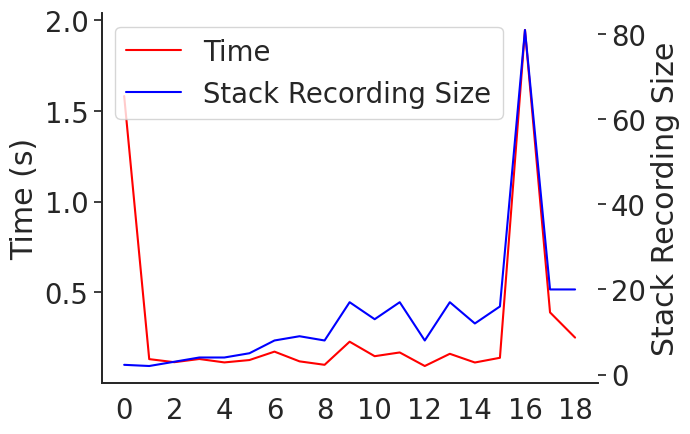
\includegraphics[width=\textwidth]{img/scenario_bs_c.png}
      \caption{\centering C}
      \label{subfig:scenario-bs-c}
  \end{subfigure}
  \hfill
  \begin{subfigure}[b]{0.45\textwidth}
      \centering
      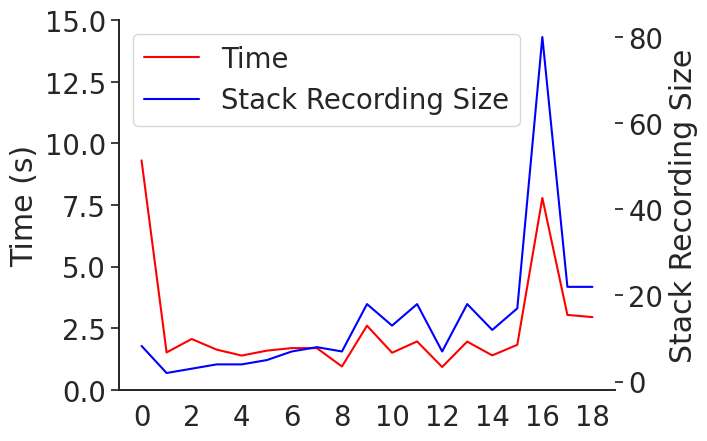
\includegraphics[width=\textwidth]{img/scenario_bs_java.png}
      \caption{\centering Java}
      \label{subfig:scenario-bs-java}
  \end{subfigure}
  \begin{subfigure}[b]{0.45\textwidth}
    \centering
    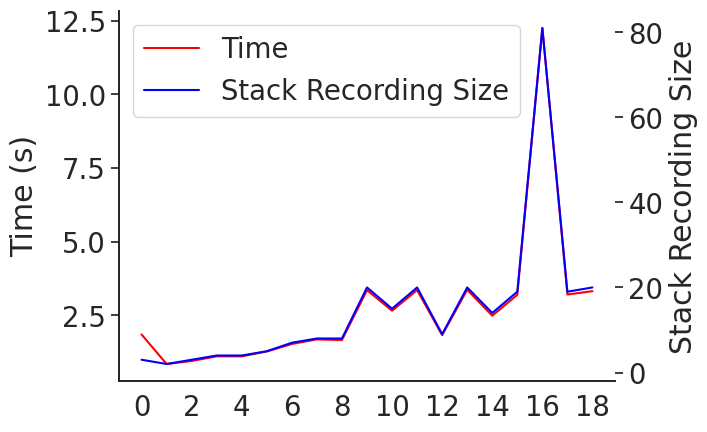
\includegraphics[width=\textwidth]{img/scenario_bs_python.png}
    \caption{\centering Python}
    \label{subfig:scenario-bs-py}
  \end{subfigure}
  \hfill
  \begin{subfigure}[b]{0.45\textwidth}
    \centering
    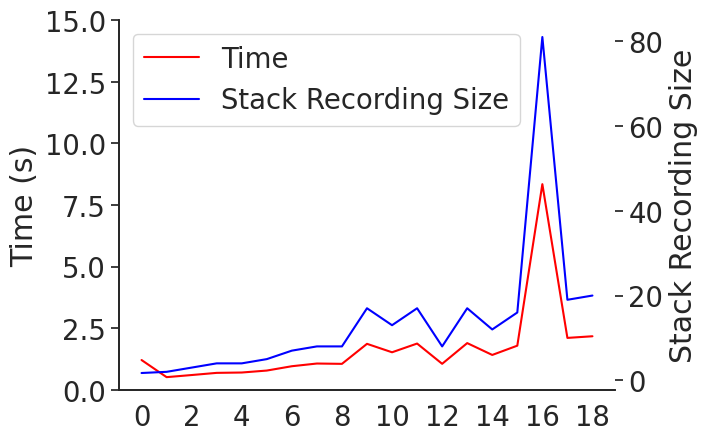
\includegraphics[width=\textwidth]{img/scenario_bs_javascript.png}
    \caption{\centering Javascript}
    \label{subfig:scenario-bs-js}
  \end{subfigure}

  \caption{Execution time and Stackrecording size for binary search scenario.}
  \label{fig:scenario-bs}
\end{figure}


To test the performance of our approach under real conditions, we recreated the live programming scenario presented in the video by bret victor. 
The scenario describes the programming of a function performing a binary search on an array of characters. It consists of 19 steps, including 10 steps where the source code is modified and 9 steps where the parameters are changed. 

\begin{table}
\begin{enumerate}
  \item The function is defined and the parameters are defined to be an array of characters(\code{['a','b','c','d','e',f']}) and a target character(\code{'d'}).
  \item A new variable \code{low} is defined.
  \item A new variable \code{high} is defined.
  \item A new variable \code{mid} is defined.
  \item The variable \code{mid} is changed to be a integer.
  \item A new variable \code{value} is defined.
  \item A if and else snippets is added.
  \item The target is changed to \code{'b'}.
  \item The target is changed to \code{'c'}.
  \item The target is changed to \code{'d'} and the code from the \code{mid} is refactored to be in a \code{while(true)} loop.
  \item The target is changed to \code{'a'}.
  \item The target is changed to \code{'b'}.
  \item The target is changed to \code{'c'}.
  \item The target is changed to \code{'d'}.
  \item The target is changed to \code{'e'}.
  \item The target is changed to \code{'f'}.
  \item The target is changed to \code{'g'}.
  \item The condition of the while loop is changed to \code{low <= high}.
  \item A return \code{-1} is added at the end of the function.
\end{enumerate}
\caption{Steps of the binary search scenario.}
\label{table:scenario-bs}
\end{table}


The scenario also includes the case where the tested method does not finish at step 17. As the code in Bret Victor's presentation is in Javascript, it has been adapted to the 3 languages studied in this paper.

For this test we set the maximum size of the stack recording at 80 stackframes. When the recording exceeds this limit, the debugger is stopped and restarted.

The figure \ref{fig:scenario-bs} shows the time and number of stackframes recorded for each stage of the scenario in Python, C, Java and Javascript. 
When the initialisation is executed for Java and C, the time taken at each stage follows the same trend as the number of stack frames registered. 
At step 16, we also observe the case of an infinite loop in the scenario.


\section{Discussion \&\ Related Work}
\label{sec:related-work}

\subsection{Discussion}

While our approach to implement live probes on top of off-the-shelf debuggers provides a viable strategy to add live probes to many mainstream languages, some limitations and open questions remain. Below discuss these in more detail.

``All problems in computer science can be solved by another level of indirection,''\footnote{Attributed to David Wheeler (\url{https://en.wikipedia.org/wiki/David_Wheeler_(computer_scientist)})} yet that often creates other problems. This state of affairs can be recognized in some of the performance results of the DAP-based live probes discussed above. Layering another level of abstraction (the DAP) between the native debuggers and the live probe server, causes performance to degrade, in this case mostly because of the asynchronous nature of the DAP, and serializing data shipped back and forth over sockets (TO CHECK). 


In our current approach, the programmer specifies input arguments to functions or methods using special comments in the code. This choice is motivated by the fact that it works in every programming language, does not require special UI affordances, and allows example data to be committed to version control systems. Nevertheless, while most primitive data types have a convenient, human readable literal notation, this can become cumbersome with complex, hetergeneous, structured data, such as arrays, objects, records, etc.  Moreover, these literal notations are language specific: how to specify a constant array in C, Java or Javascript is very different, and needs to be parsed into actual data values from their textual representation in the special comments. 

Another challenge is most visible in the case of object-oriented languages, such as Java, where methods typically live in classes, and can only be invoked when an instance of a class is available. This means the programmer has to specify not just the input parameters, but also values for fields, or arguments to constructors, so that the live probe server can construct the object. This situation becomes worse if, e.g., the constructor depends on other objects as argument, which, in turn, require initialization, and so on. At minimum, the live probe server could construct basic objects with default values for all constructor arguments, and let the programmer gradually modify improve the assignment using annotations. 

The above problem of objects and initialization hints at a more basic and general question: how to obtain useful example data in the first place. In this paper we have assumed the programmer provides the data, but there are other strategies worth considering. For instance:
\begin{itemize}
  \item As a base case, one could use default values for all arguments (e.g., \lstinline{0}, \lstinline{""}, \lstinline{null}, etc.). This has the drawback that such values might not lead to interesting probe displays. 
  \item Random value generation, as is employed in randomized testing, could be used to assign values to parameters. However, in this case it is unclear if it leads to the insight the programmer wants, and would be very confusing if the values would change in every iteration.
  \item If a test suite is available, an off-line tool could observe frequently occurring values and objects passed into methods, through dynamic analysis of the test suite execution. Such common values could also be harvested from production runs. Just like with random generation, however, the problem is to make the assignments stable somehow. 
\end{itemize}
The above strategies absolve the programmer from having to specify the example values, but potentially at the cost of reduced quality of feedback. Further research is needed to find an appropriate middle ground between full manual specification, and fully automatic techniques.

Live probes require continual execution of methods and functions. This is fine if the code does not perform any harmful side-effects, such as sending out email, writing files, or launching missiles. While it is probably undecidable to statically check whether a piece of code might eventually perform such a side effect, we leave it to the programmer to indicate whether the live probing feature is switched on, e.g., by providing the annotation of the input arguments. 

Possible future directions to solve this problem would include sandboxed execution~\cite{???}, or intercepting all calls to IO libraries or the operating system. The latter technique would also allow the live probes to not only display variable values, but also, e.g., console output. 
A more disciplined solution would be offered by languages with built-in notions of capability-based security (such as, e.g., Newspeak~\cite{Newspeak}), so that the live probes can be configured to execute in an environment where dangerous features (such as IO) are not available.  

While the live probes that we have demonstrated support variables updated in loops by displaying them in tabular form, we have not discussed what happens with recursion. The live probe execution repeatedly instructs the debugger to step-over function calls, intermediate stack frames are automatically excluded from the stack-recording, \textit{except} for execution arrives back at the function that is currently probed, since it has a breakpoint on entry. Our current implementation simply continues, and adds stack frames to the recording, even though we are on a different level of the stack. Further research is needed to explicitly deal with this case, and find an appropriate tree-based or nested visualization.

\subsection{Related Work}

Example-Based Live Programming for Everyone\cite{ExampleBasedGraalVM} : Use GraalVM/Truffle to get live information from the code of multiple languages.

Example Centric Programming\cite{ExampleCentric} : Use BeanShell(custom JVM) to get live information. Prototype for Java in Eclipse.

Usable Live Programming\cite{UsableLiveProgramming} : New language for live programming(Ying Yang) with incremental compilation. Live programming environment for this language.
Use source location to relate execution and code(=> almost like stack recording that link stackframe and code location)

Scalable Omniscient Debugging\cite{ScalableOmniscient} : Omniscient debugging with a lot of data. Use a lot of memory to store all the data.
In this paper they record almost everything, we only record the stackframe.

LiveLiterals~\cite{LiveLiterals}

\section{Conclusion}
\label{sec:conclusion}

\printbibliography

\end{document}

% Local Variables:
% TeX-engine: luatex
% End:
